
\chapter{Rates}


%94. 
\section{The derivative considered as the ratio of two rates}

Let

\[
    y = f(x)
\]
be the equation of a curve generated by a moving point P. 
Its coordinates $x$ and $y$ may then be considered as functions 
of the time, as explained in \S \ref{sec:71}. %§ 71, p. 91.
Differentiating with respect to $t$, by the chain rule 
(Formula XXV in \S \ref{sec:33}), we have

\begin{equation}
%(32) 
\frac{dy}{dt} = f'(x) \frac{dx}{dt}.
\label{eqn:32-94}
\end{equation}
{\it At any instant the time rate of change of $y$ (or the function) 
equals its derivative multiplied by the time rate change of the 
independent variable.}

Or, write (\ref{eqn:32-94}) in the form

\[
%(33) 
\frac{\frac{dy}{dt}}{\frac{dx}{dt}} = f'(x) = \frac{dy}{dx}.
\]
{\it The derivative measures the ratio of the time rate of 
change of $y$ to that of $x$.}

\begin{figure}[h!]
%\begin{tabular}{cc}
\begin{minipage}{\textwidth}
\begin{center}
%\vspace{1.0 cm}
%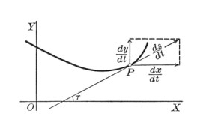
\includegraphics[height=3cm,width=6cm]{two-rates.eps}
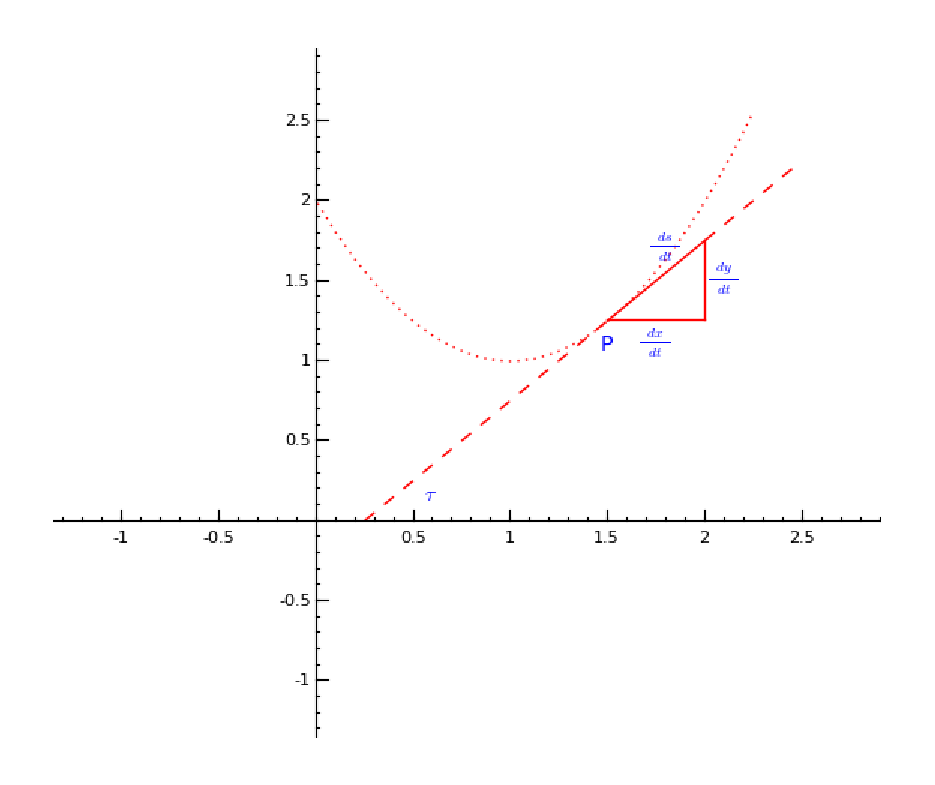
\includegraphics[height=5cm,width=8cm]{arclength.eps}
\end{center}
\end{minipage}
%\caption{Scan of Granville's graphic of the derivative the arc length.}
\caption{Geometric visualization of the derivative the arc length.}
\label{fig:two-rates}
\end{figure}
%sage: p1 = plot(1+(x-1)^2, 0,2.25, rgbcolor=(0,0,0))
%sage: p1a = plot(1+(x-1)^2, 0, 2.25, rgbcolor=(1,0,0), linestyle=":")
%sage: p2a = plot(x-1/4, 0.25, 1.5, rgbcolor=(1,0,0), linestyle="--")
%sage: p2b = plot(x-1/4, 1.5, 2.5, rgbcolor=(1,0,0))
%sage: p2c = plot(x-1/4, 2, 2.5, rgbcolor=(1,0,0), linestyle="--")
%sage: p3 = line([[1.5,1.25],[2.0,1.25]], rgbcolor=(1,0,0))
%sage: p4 = line([[2.0,1.25],[2.0,1.75]], rgbcolor=(1,0,0))
%sage: t1 = text("P", (1.5,1.1))
%sage: t1 = text("P", (1.5,1.0))
%sage: t2 = text("$\\tau$", (0.6, 0.15))
%sage: t3 = text("$\\frac{dx}{dt}$", (1.75, 1.1))
%sage: t4 = text("$\\frac{dy}{dt}$", (2.1, 1.5))
%sage: t5 = text("$\\frac{ds}{dt}$", (1.8, 1.7))
%sage: show(p1a+p2a+p2b+p2c+p3+p4+t1+t2+t3+t4+t5,tick_color=(1,0,0))

\noindent
$\frac{ds}{dt}$ being the time rate of change of length 
of arc, we have from (\ref{eqn:12-71}), % p. 92 [§71],

\begin{equation}
%(34) 
\frac{ds}{dt} 
= \sqrt{\left ( \frac{dx}{dt} \right )^2 + \left ( \frac{dt}{dt} \right )^2}.
\label{eqn:34-94}
\end{equation}
which is the relation indicated by Figure \ref{fig:two-rates}.

As a guide in solving rate problems use the following rule:

\begin{itemize}
\item
FIRST STEP. Draw a figure illustrating the problem. 
Denote by $x$, $y$, $z$, etc., the quantities which vary with the time.

\item
SECOND STEP. Obtain a relation between the variables 
involved which will hold true at any instant.

\item
THIRD STEP. Differentiate with respect to the time.

\item
FOURTH STEP. Make a list of the given and required quantities.

\item
FIFTH STEP. Substitute the known quantities in the result 
found by differentiating (third step), and solve for the unknown.
\end{itemize}



\section{Exercises}


\begin{enumerate}

\item
%1
A man is walking at the rate of $5$ miles per hour towards the foot 
of a tower $60$ ft. high. At what rate is he approaching the 
top when he is $80$ ft. from the foot of the tower?

Solution. Apply the above rule.

First step. Draw the figure. Let $x$ = distance of the man from 
the foot and $y$ = his distance from the top of the tower at any instant.

Second step. Since we have a right triangle,
$\ y^2 	= x^2 + 3600$.

Third step. Differentiating, we get
$2 y \frac{dy}{dt} 	= 2 x \frac{dx}{dt}$, or,
%(A) 
$\frac{dy}{dt} 	= \frac{x}{y} \frac{dx}{dt}$, 
meaning that at any instant whatever
(Rate of change of $y$) = $\left ( \frac{x}{y} \right )$ 
(rate of change of $x$).

Fourth step. 

\[
\begin{array}{ll}
 x &	= 80,\ 	\frac{dx}{dt} 	= 5\ {\rm miles/hour},\\
  &= 5 \times 5280 ft/hour,\\
y &	= \sqrt{x^2 + 3600}\\
  &	= 100.\\
 \frac{dy}{dt}& 	= ?
\end{array}
\]
Fifth step. 	Substituting back in the above %(A),
$\frac{dy}{dt} 	= \frac{80}{100} \times 5 \times 5280$
ft/hour = $4$ miles/hour. 

\item
%2
A point moves on the parabola $6y = x^2$ in such a way that when 
$x = 6$, the abscissa is increasing at the rate of $2$ ft. per second. 
At what rates are the ordinate and length of arc increasing at the 
same instant?

Solution. First step. Plot the parabola.

Second step. $6 y 	= x^2$.

Third step. $6 \frac{dy}{dt} 	= 2 x\frac{dx}{dt}$, or,
%(B) 	
$\frac{dy}{dt} 	= \frac{x}{3} \cdot \frac{dx}{dt}$.
This means that at any point on the parabola
(Rate of change of ordinate) 	
= $\left( \frac{x}{3} \right)$ (rate of change of abcissa).

Fourth step. $\frac{dx}{dt} 	= 2$ ft. per second,
$x = 6$, $\frac{dy}{dt} = ?$, 
$y = \frac{x^2}{6} = 6$, $\frac{ds}{dt} = ?$

Fifth step. Substituting back in the above, %(B),
$\frac{dy}{dt} = \frac{6}{3} \times 2 = 4$ ft. per second. 

From the first result we note that at the point 
$(6, 6)$ the ordinate changes twice as rapidly as the abscissa.

If we consider the point $(-6, 6)$ instead, the result is 
$\frac{dy}{dt} = -4$ ft. per second, the minus sign indicating 
that the ordinate is decreasing as the abscissa increases.

We shall now solve this using \sage.

\vskip .1in

{\scriptsize{
\begin{Verbatim}[fontsize=\small,fontfamily=courier,fontshape=tt,frame=single,label=\sage]

sage: t = var("t")
sage: x = function("x",t)
sage: y = function("y",t)
sage: eqn = 6*y - x^2
sage: solve(diff(eqn,t) == 0, diff(y(t), t, 1))
[diff(y(t), t, 1) == x(t)*diff(x(t), t, 1)/3]
sage: s = sqrt(x^2+y^2)
sage: diff(s,t)
(2*y(t)*diff(y(t), t, 1) 
  + 2*x(t)*diff(x(t), t, 1))/(2*sqrt(y(t)^2 + x(t)^2))

\end{Verbatim}
}}
\vskip .1in

\noindent
This tells us that 
$\frac{dy}{dt} =\frac{x}{3} \cdot \frac{dx}{dt}$ and

\[
\frac{ds}{dt} =\frac{ y(t)y'(t) +  x(t)x'(t)}{\sqrt{ x(t)^2  + y(t)^2}}.
\]
Substituting $\frac{dx}{dt} = 2$, $x = 6$, gives
$\frac{dy}{dt} = 4$. In addition, if $y=6$ then this gives
$\frac{ds}{dt} = 36/\sqrt{72}=3\sqrt{2}$.

\item
%3
A circular plate of metal expands by heat so that its radius 
increases uniformly at the rate of $0.01$ inch per second.
At what rate is the surface increasing when the radius is two inches?

Solution. Let $x$ = radius and y = area of plate. Then
$ y 	= \pi x^2$,
%(C) 	
$\frac{dy}{dt} 	= 2 \pi x \frac{dx}{dt}$,
That is; at any instant the area of the plate is increasing 
in square inches $2\pi x$ times as fast as the radius is 
increasing in linear inches.
$\ x 	= 2$, $\frac{dx}{dt} = 0.01$, 
$\frac{dy}{dt} = ?$.
Substituting in the above, %(C),
$\frac{dy}{dt} 	= 2 \pi \times 2 \times 0.01 = 0.04 \pi$ 
sq. in. per sec. 

\item
%4
An arc light is hung $12$ ft. directly above a straight 
horizontal walk on which a boy $5$ ft. in height is walking. 
How fast is the boy's shadow lengthening when he is walking 
away from the light at the rate of 168 ft. per minute?

Solution. Let $x$ = distance of boy from a point directly 
under light $L$, and $y$ = length of boy's shadow. 
By similar triangle, %From the figure,
$y/( y + x) = 5/12$,
or $ y 	= \frac{5}{7} x$.
Differentiating, $\frac{dy}{dt} = \frac{5}{7} \frac{dx}{dt}$;
i.e. the shadow is lengthening $\frac{5}{7}$ as fast as 
the boy is walking, or $120$ ft. per minute.

\item
%5
In a parabola $y^2 = 12x$, if $x$ increases uniformly at 
the rate of $2$ in. per second, at what rate is $y$ increasing 
when $x = 3$ in. ? 

Ans. $2$ in. per sec.

\item
%6
At what point on the parabola of the last example do the 
abscissa and ordinate increase at the same rate? 

Ans. $(3,6)$.

\item
%7
In the function $y = 2x^3 + 6$, what is the value of $x$ at the 
point where $y$ increases $24$ times as fast as $x$? 

Ans. $x = \pm 2$.

\item
%8
The ordinate of a point describing the curve 
$x^2 + y^2 = 25$ is decreasing at the rate of $3/2$ in. per second. 
How rapidly is the abscissa changing when the ordinate is $4$ inches? 

Ans. $\frac{dx}{dt} = 2$ in. per sec.

\item
%9
Find the values of $x$ at the points where the rate of change of
$ x^3 - 12x^2 + 45x - 13$
is zero. 

Ans. $x = 3$ and $5$.

\item
%10
At what point on the ellipse $16x^2 + 9y^2 = 400$ does $y$ decrease 
at the same rate that $x$ increases? 

Ans. $(3, \frac{16}{3})$.

\item
%11
Where in the first quadrant does the arc increase twice as 
fast as the ordinate? 

Ans. At $60^o = \pi/3$.

\end{enumerate}

A point generates each of the following curves (problems 12-16). 
Find the rate at which the arc is increasing in each case:

\begin{enumerate}
\addtocounter{enumi}{11}

\item
%12
$y^2 = 2x$; $\frac{dx}{dt} = 2$, $x = 2$. 	

Ans. 	
$\frac{ds}{dt} = \sqrt{5}$.

\item
%13
$xy = 6$; $\frac{dy}{dt} = 2$, $y = 3$. 

Ans. $\frac{ds}{dt} = \frac{2}{3} \sqrt{13}$.

\item
%14
$x^2 + 4 y^2 = 20$; $\frac{dx}{dt} = - 1$, $y = 1$.

Ans. $ 	\frac{ds}{dt} = \sqrt{2}$.

\item
%15
$y = x^3$; $\frac{dx}{dt} = 3$, $x = - 3$.

\item
%16
$y^2 = x^3$; $\frac{dy}{dt} = 4$, $y = 8$.

\item
%17
The side of an equilateral triangle is $24$ inches long, and is 
increasing at the rate of $3$ inches per hour. 
How fast is the area increasing? 

Ans. $36\sqrt{3}$ sq. in. per hour.

\item
%18
Find the rate of change of the area of a square when the side 
$b$ is increasing at the rate of $a$ units per second. 

Ans. $2 ab$ sq. units per sec.

\item
%19
(a) The,volume of a spherical soap bubble increases how 
many times as fast as the radius? 
(b) When its radius is $4$ in. and increasing at the rate of 
$1/2$ in. per second, how fast is the volume increasing? 

Ans. (a) $4\pi r^2$ times as fast; (b) $32\pi$ cu. in. per sec.

How fast is the surface increasing in the last case?

\item
%20
One end of a ladder $50$ ft. long is leaning against a 
perpendicular wall standing on a horizontal plane. Supposing 
the foot of the ladder to be pulled away from the wall at 
the rate of $3$ ft. per minute; 
(a) how fast is the top of the ladder descending when 
the foot is $14$ ft. from the wall? 
(b) when will the top and bottom of the ladder move at the same rate? 
(c) when is the top of the ladder descending at the 
rate of $4$ ft. per minute? 

Ans. (a) $\frac{7}{78}$ ft. per min.; 
(b) when $25 \sqrt{2}$ ft. from wall; 
(c) when $40$ ft. from wall.

\item
%21
A barge whose deck is $12$ ft. below the level of a dock is drawn 
up to it by means of a cable attached to a ring in the 
floor of the dock, the cable being hauled in by a windlass 
on deck at the rate of $8$ ft. per minute. 
How fast is the barge moving towards the dock when $16$ ft. away? 

Ans. $10$ ft. per minute.

\item
%22
An elevated car is $40$ ft. immediately above a surface car, their 
tracks intersecting at right angles. If the speed of the elevated 
car is $16$ miles per hour and of the surface car $8$ miles per hour, 
at what rate are the cars separating $5$ minutes after they meet? 

Ans. $17.9$ miles per hour.

\item
%23
One ship was sailing south at the rate of $6$ miles per hour; another 
east at the rate of $8$ miles per hour. At $4$ P.M. the second 
crossed the track of the first where the first was two hours 
before; (a) how was the distance between the ships changing 
at $3$ P.M.? (b) how at $5$ P.M.? (c) when was the distance between 
them not changing? 

Ans. (a) Diminishing $2.8$ miles per hour; 
(b) increasing $8.73$ miles per hour; (c) $3: 17$ P.M.

\item
%24
Assuming the volume of the wood in a tree to be proportional 
to the cube of its diameter, and that the latter increases 
uniformly year by year when growing, show that the rate of growth 
when the diameter is $3$ ft. is $36$ times as great as when the 
diameter is $6$ inches.

\item
%25
A railroad train is running 15 miles an hour past a station 
$800$ ft. long, the track having the form of the parabola
$ y^2 = 600x$,
and situated as shown in Figure \ref{fig:train}. 

\begin{figure}[h!]
%\begin{tabular}{cc}
\begin{minipage}{\textwidth}
\begin{center}
%\vspace{1.0 cm}
%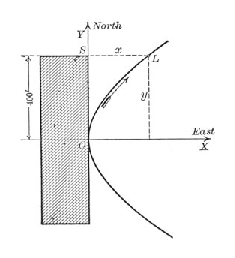
\includegraphics[height=3cm,width=6cm]{train.eps}
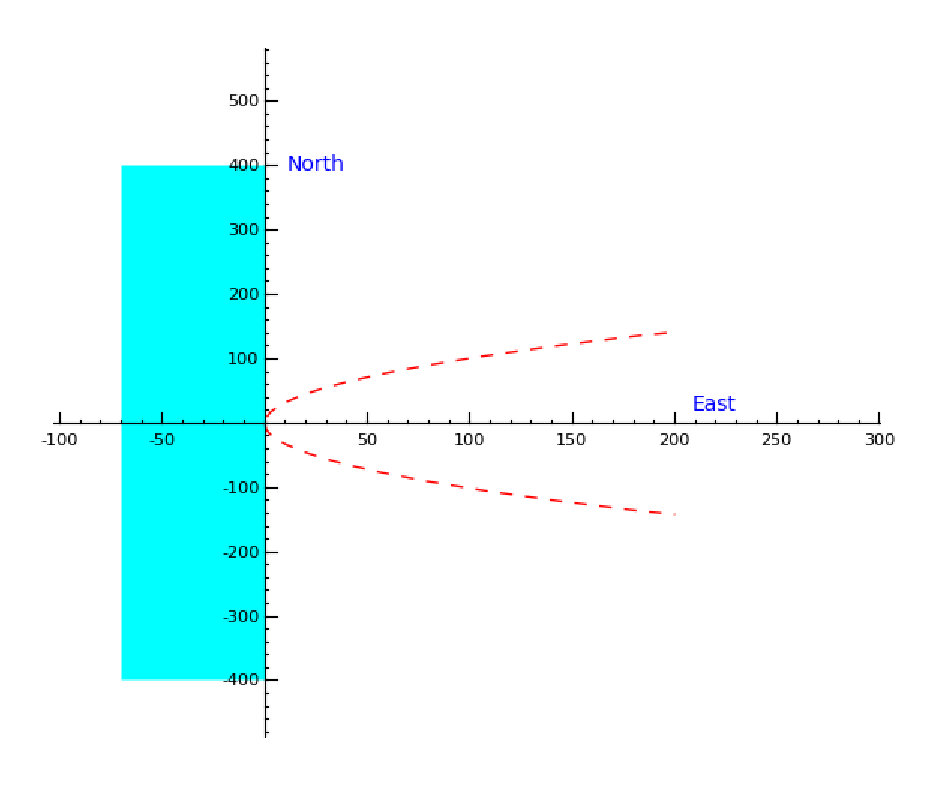
\includegraphics[height=5cm,width=7cm]{train-station.eps}
\end{center}
\end{minipage}
%\caption{Scan of Granville's graphic of the train's trajectory.}
\caption{Train station and the train's trajectory.}
\label{fig:train}
\end{figure}


If the sun is just rising in the east, find how fast the shadow 
$S$ of the locomotive $L$ is moving along the wall of the station 
at the instant it reaches the end of the wall.

Solution. $y^2 	= 600x$,
$2 y \frac{dy}{dt} 	= 600 \frac{dx}{dt}$,
or $\frac{dx}{dt} 	= \frac{y}{300} \frac{dy}{dt}$.
Substituting this value of $\frac{dx}{dt}$ in
$\frac{ds}{dt} 	
= \sqrt{\left( \frac{dx}{dt} \right)^2 
+ \left( \frac{dy}{dt} \right)^2}$, we get
%(D) 	
$\left( \frac{ds}{dt} \right)^2 
= \left( \frac{y}{300} \frac{dy}{dt} \right)^2 
+ \left( \frac{dy}{dt} \right)^2$.
Now $\frac{ds}{dt} 	= 15$ miles per hour = $22$ ft. per sec.,
$y= 400$ and $\frac{dy}{dt} = ?$.
Substituting back in the above, %(D), 
we get
$
 ( 22 )^2 	
= \left( \frac{16}{9} + 1 \right) \left( \frac{dy}{dt} \right)^2$,
or, 
$\frac{dy}{dt} 	
= 13 \frac{1}{5}$ ft. per second. 

\item
%26
An express train and a balloon start from the same point at 
the same instant. The former travels $50$ miles an hour and the 
latter rises at the rate of $10$ miles an hour. How fast are 
they separating? 

Ans. $51$ miles an hour.

\item
%27
A man $6$ ft. tall walks away from a lamp-post $10$ ft. high at 
the rate of $4$ miles an hour. How fast does the shadow of his 
head move? 

Ans. $10$ miles an hour.

\item
%28
The rays of the sun make an angle of $30^o = \pi/6$ with the 
horizon. A ball is thrown vertically upward to a height 
of $64$ ft. How fast is the shadow of the ball moving along 
the ground just before it strikes the ground? 

Ans. $110.8$ ft. per sec.

\item
%29
A ship is anchored in $18$ ft. of water. The cable passes over 
a sheave on the bow $6$ ft. above the surface of the water. If 
the cable is taken in at the rate of $1$ ft. a second, how fast 
is the ship moving when there are $30$ ft. of cable out? 

Ans. $\frac{5}{3}$ ft. per sec.

\item
%30
A man is hoisting a chest to a window $50$ ft. up by means of 
a block and tackle. If he pulls in the rope at the rate of $10$ ft. 
a minute while walking away from the building at the rate of 
$5$ ft. a minute, how fast is the chest rising at the end of the 
second minute? 

Ans. $10.98$ ft. per min.

\item
%31
Water flows from a faucet into a hemispherical basin of 
diameter $14$ inches at the rate of $2$ cu. in. per second. 
How fast is the water rising (a) when the water is halfway to 
the top? (b) just as it runs over? (The volume of a 
spherical segment = $\frac{1}{2} \pi r^2 h + \frac{1}{6} \pi h^3$, 
where $h$ = altitude of segment.)

\item
%32
Sand is being poured on the ground from the orifice of an 
elevated pipe, and forms a pile which has always the shape of a 
right circular cone whose height is equal to the radius of the 
base. If sand is falling at the rate of $6$ cu. ft. per sec., 
how fast is the height of the pile increasing when the height is $5$ ft.?

\item
%33
An aeroplane is $528$ ft. directly above an automobile and starts 
east at the rate of $20$ miles an hour at the same instant the 
automobile starts east at the rate of $40$ miles an hour. 
How fast are they separating?

\item
%34
A revolving light sending out a bundle of parallel rays is at 
a distance of $t$ a mile from the shore and makes $1$ revolution a 
minute. Find how fast the light is traveling along the straight 
beach when at a distance of $1$ mile from the nearest point of 
the shore. 

Ans. $15.7$ miles per min.

\item
%35
A kite is $150$ ft. high and $200$ ft. of string are out. If the 
kite starts drifting away horizontally at the rate of $4$ 
miles an hour, how fast is the string being paid out at 
the start? 

Ans. $2.64$ miles an hour.

\item
%36
A solution is poured into a conical filter of base radius $6$ cm. 
and height $24$ cm. at the rate of $2$ cu. cm. a second, and 
filters out at the rate of $1$ cu. cm. a second. 
How fast is the level of the solution rising when 
(a) one third of the way up? (b) at the top? 

Ans. (a) $0.079$ cm. per sec.; (b) $0.009$ cm. per sec.

\item
%37
A horse runs $10$ miles per hour on a circular track in the 
center of which is an arc light. How fast will his shadow move 
along a straight board fence (tangent to the track at the 
starting point) when he has completed one eighth of the 
circuit? 

Ans. $20$ miles per hour.

\item
%38
The edges of a cube are $24$ inches and are increasing at the 
rate of $0.02$ in. per minute. At what rate is 
(a) the volume increasing? 
(b) the area increasing?

\item
%39
The edges of a regular tetrahedron are $10$ inches and are 
increasing at the rate of $0.3$ in. per hour. At what rate 
is (a) the volume increasing? (b) the area increasing?

\item
%40
An electric light hangs $40$ ft. from a stone wall. A man is 
walking $12$ ft. per second on a straight path $10$ ft. from 
the light and perpendicular to the wall. How fast is the man's 
shadow moving when he is $30$ ft. from the wall? 

Ans. $48$ ft. per sec.

\item
%41
The approach to a drawbridge has a gate whose two arms 
rotate about the same axis as shown in the figure. The arm 
over the driveway is $4$ yards long and the arm over the footwalk 
is $3$ yards long. Both arms rotate at the rate of $5$ radians 
per minute. At what rate is the distance between the 
extremities of the arms changing when they make an angle 
of $45^o=\pi/4$ with the horizontal? 

Ans. $24$ yd. per min.

\item
%42
A conical funnel of radius $3$ inches and of the same depth 
is filled with a solution which filters at the rate of $1$ cu. in. 
per minute. How fast is the surface falling when it is $1$ 
inch from the top of the funnel? 

Ans. $\frac{1}{4 \pi}$ in. per mm.

\item
%43
An angle is increasing at a constant rate. Show that the 
tangent and sine are increasing at the same rate when the 
angle is zero, and that the tangent increases eight times 
as fast as the sine when the angle is $60^o=\pi/3$.

\end{enumerate}
